\chapter{Quanten-Teleportation\label{chapter:teleport}}
\lhead{Quanten-Teleportation}
\begin{refsection}
\chapterauthor{Max Obrist und Martin Stypinski}

\section{Einleitung}
Die Quantenteleportation beschreibt die M"oglichkeit Quantenzust"ande "uber eine Distanz zu transportieren. Die Kernidee bei der Quantenteleportation ist nicht die "ubertragung von Quanten, sondern viel mehr die "ubertragung der Information. Ein Quantenzustand soll quasi von A nach B transportiert werden. Die Information soll "uber einen 'Informationskanal' "ubertragen werden, die Quanten an sich, da sie sehr schnell den Zustand "andern, aber werden im eigentlichen Sinne nicht "ubertragen.

\section{Problem}
\subsection{Klassische Kommunikation}
Angefangen bei der klassischen Kommunikation kann man die Informations"ubertragung sehr einfach darstellen. Der Sender Alice verpackt seine Information in eine Kiste. Diese wird mittels einem Speditionsunternehmen zu Bob transportiert. Bob "offnet die Kiste und findet die Information wieder. Die Kommunikation zwischen Alice und Bob konnte somit stattfinden. Dies ist sehr einfach und anschaulich erkl"art und ben"otigt eine 'physische' "ubertragung der Information. Einfacher ist es mit einem Faxger"at. Der Sender Alice faxt seine Meldung zu Empf"anger Bob. Alice und Bob haben somit Informationen ausgetauscht.
\begin{figure}
\center
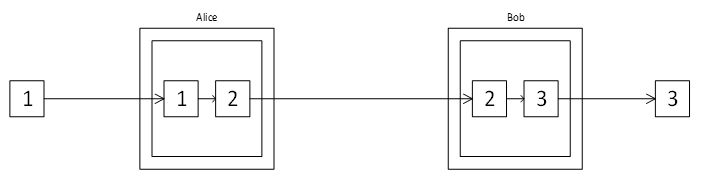
\includegraphics[width=0.75\textwidth]{teleport/image/classic_communication.png}
\caption{Klassische Kommunikation von Alice zu Bob.}
\label{Klassische Kommunikation}
\end{figure}
\subsection{Quantenmechanisches Problem}
Das Problem in der Quanteninformatik ist, dass der Zustand eines Teilchens nicht ohne weiteres von Alice zu Bob "ubertragen werden kann. Besitzt Alice ein Teilchen im Zustand $\left|\phi\right\rangle$ kann sie dessen Zustand nicht ohne weiteres an Bob "ubertragen. Der naive Versuch einfach das Teilchen zu "ubertragen, birgt verschiedene technische Schwierigkeiten mit sich. Es ist "ausserst schwierig, ein Teilchen unver"andert "uber gr"ossere Distanzen zu transportieren. F"ur den gesamten Transportweg m"ussten s"amtliche Wechselwirkungen eliminiert werden. 
\\
Die Heisenbergschen Unsch"arferelation zeigt ausserdem, dass es Alice unm"oglich ist, das zu "ubertragende Teilchen so zu messen, dass Bob daraus den Originalzustand rekonstruieren k"onnte (Reduktionspostulat). Nehmen wir zur Illustration die Polarisationsrichtung eines Photons. Das Photon befindet sich in einem Zustand $\left|\phi\right\rangle$, welcher eine Superposition aus den Zust"anden $\leftrightarrow$ (horizontal polarisiert) und $\updownarrow$(vertikal polarisiert) besteht. Das System $\left|\phi\right\rangle$ l"asst sich somit formal schreiben als
\begin{align}\label{eq:qubit1}
\left|\phi\right\rangle = \alpha\left|\leftrightarrow\right\rangle + \beta\left|\updownarrow\right\rangle 
\end{align}
mit $\alpha, \beta \in \mathbb{C}$ und der Bedingung $\left|\alpha\right|^{2} + \left|\beta\right|^{2} = 1$. Im folgenden verwenden wir die "ublichere Notation f"ur 2-Zustandsysteme und schreiben die beiden Zust"ande als $\left| 0 \right\rangle$ (horizontal polarisiert) und $\left| 1 \right\rangle$ (vertikal polarisiert). Das auch unter dem Namen Qubit bekannte System l"asst sich dann schreiben als 
\begin{align}\label{eq:qubit2}
\left|\phi\right\rangle = \alpha\left|0\right\rangle + \beta\left|1\right\rangle.
\end{align}
Misst man nun ein System, welches mit Gleichung~\ref{eq:qubit1} beschrieben wird, hat eine Messung der Spinkomponente folgende Wahrscheinlichkeiten:
\begin{align}
	\begin{split}
		W\left(\leftrightarrow\right) & =\left|\alpha\right|^2  \\
	    W\left(\updownarrow\right) & =\left|\beta\right|^2
	\end{split}
\end{align}
F"uhrt man eine Messung von $\alpha$ oder $\beta$ durch, wird die Superposition des Teilchens zerst"ort und es befindet sich in einem der Basiszust"ande $\updownarrow$ oder $\leftrightarrow$. Die jeweils andere Komponente l"asst sich nun nicht mehr bestimmen. Es scheint also unm"oglich, den vollst"andigen Zustand eines Teilchens mit einer Messung zu bestimmen.
\section{L"osung}
Auch wenn die heisenbergsche Unsch"arferelation dem Vorhaben von Alice, eine Teilchen zu Bob zu schicken, auf den ersten Blick im Wege steht, ist es genau dasselbe Prinzip, welche bei der Quantenteleportation – zusammen mit der Quantenverschr"ankung – eine zentrale Rolle spielt.
\begin{figure}
	\center
	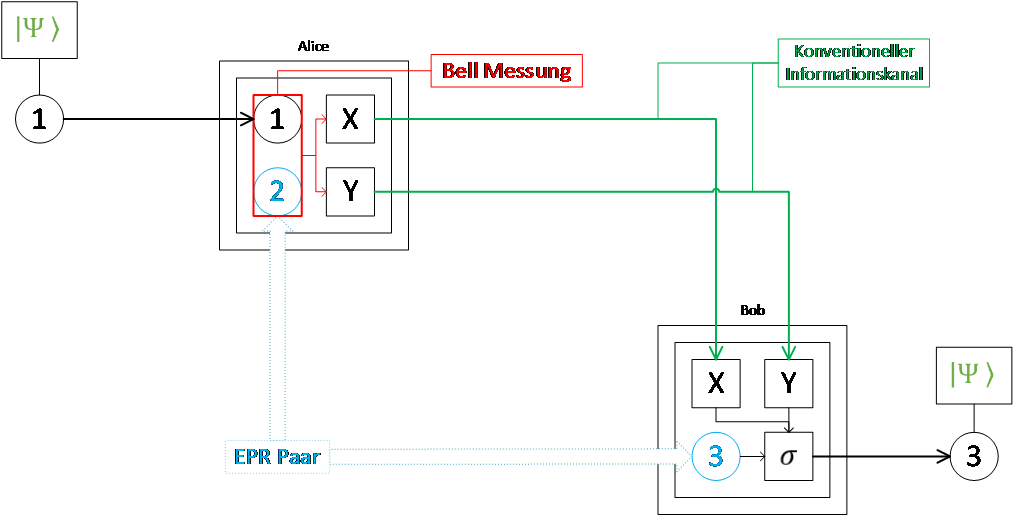
\includegraphics[width=1\textwidth]{teleport/image/quantum_teleportation.png}
	\caption{Quantenteleportation}
	\label{Quantenteleportation}
\end{figure}

Voraussetzung f"ur den Quantenteleporationsprozess ist, dass Alice und Bob je ein Teilchen eines verschr"ankten EPR-Paares besitzen, die Teilchen $T_{2}$ und $T_{3}$. Ein EPR-Paar ist ein verschr"anktes System mit zwei Teilchen, welches sich in einem der vier Bell Zust"ande befindet. F"ur unser Beispiel nehmen wir an, dass sich das Paar in folgendem Zustand befindet:
\begin{align}\label{eq:bell_state1}
\left|\Psi^{-}\right\rangle_{23} = \frac{1}{\sqrt{2}} ( \left|0\right\rangle_{2}\left|1\right\rangle_{3} - \left|1\right\rangle_{2}\left|0\right\rangle_{3} )
\end{align}
\\
Dieser Zustand erlaubt keinerlei R"uckschl"usse auf den eigentlichen Zustand von $T_{2}$ und $T_{3}$. Er sagt einzig aus, dass sich $T_{2}$ und $T_{3}$ in orthogonalen Zustanden befinden. Aus einer Messung von $T_{2}$ l"asst sich der Zustand von $T_{3}$ bestimmen, zerst"ort aber gleichzeitig den Zustand von $T_{2}$. 
\\
Nun erh"alt Alice ein Teilchen $T_{1}$ im unbekannten Zustand $\left|\phi\right\rangle = \alpha\left|0\right\rangle + \beta\left|1\right\rangle$. Sie f"uhrt nun eine sogenannte Bellsche Zustandsmessung auf $T_{1}$ und $T_{2}$ durch (Eine Bellsche Zustandsmessung ist die Projektion eines beliebigen verschr"ankten Zustandes zweier Teilchen auf eine Basis mit vier Zust"anden, die Bell’sche Basis - siehe n"achster Abschnitt). 
\\
Diese Messung hat zwei Effekte. Einerseits erhalten wir als Ergebnis einen der vier Bell States. Andererseits sind nun die Teilchen $T_{1}$ und $T_{2}$ ebenfalls miteinander verschr"ankt, was bedeutet, dass $T_{1}$ seinen Zustand „verliert“ und nur noch gemeinsam mit $T_{2}$ beschreibbar ist. Der Zustand von $T_{1}$ und $T_{2}$ l"asst sich genau mit dem in der Messung erhaltenen Bell State beschreiben. Gleichzeitig sind auch die Teilchen $T_{2}$ und $T_{3}$ noch miteinander verschr"ankt, und zwar im Zustand der in Gleichung~\ref{eq:bell_state1} beschrieben ist. Wie erw"ahnt handelt es sich auch bei dieser Gleichung um einen Bellschen Zustand.
\\
Nehmen wir nun an, die Bellsche Zustandsmessung bei Alice hat als Ergebnis den folgenden Zustand:
\begin{align}\label{eq:bell_state2}
\left|\Psi^{-}\right\rangle_{12} = \frac{1}{\sqrt{2}} ( \left|0\right\rangle_{1}\left|1\right\rangle_{2} - \left|1\right\rangle_{1}\left|0\right\rangle_{3} )
\end{align}
Die Teilchen $T_{1}$ und $T_{2}$ befinden sich also im selben Bell State $\left| \Psi^{-} \right \rangle$ wie $T_{2}$ und $T_{3}$ und sind damit ebenfalls orthogonal zueinander. Nun existiert folgende Situation: $T_{1}$ und $T_{2}$ sind miteinander Verschr"ankt und befinden sich im Zustand Gleichung~\ref{eq:bell_state2}, sind also orthogonal ausgerichtet. $T_{2}$ und $T_{3}$ sind ebenfalls miteinander verschr"ankt und befinden sich im Zustand Gleichung~\ref{eq:bell_state1}, sind also ebenfalls orthogonal zueinander. Dies bedeutet, dass sich die Teilchen $T_{1}$ und $T_{3}$ - abgesehen von einem unwichtigen Phasenvektor - im selben Zustand befinden m"ussen: $\left| \Psi\right\rangle_{3} = -\left|\phi\right\rangle$
\section{Bellsche Zustandsmessung \& Bell States}
Im vorherigen Abschnitt wurde das grunds"atzliche Konzept der Quantenteleportation erl"autert. Dabei wurde allerdings die Bellsche Zustandsmessung bewusst weggelassen. Diese ist "ausserst zentral bei der Quantenteleportation, wird doch dabei einerseits das zu teleportierende Teilchen mit T2 verschr"ankt, welches sich Alice und Bob teilen. Andererseits ergibt sie als Resultat auch den Bell Zustand, in welchem sich die Teilchen T1 und T2 befinden, was es Bob erst erlaubt, den urspr"unglichen Zustand in T3 wiederherzustellen. Die Bellsche Zustandsmessung stellt sich auch bei der experimentellen Realisierbarkeit als "ausserst Komplex heraus, darauf wird in diesem Rahmen aber nicht eingegangen.
\\
Das Resultat der Bell Messung ist einer der vier Bell States. Diese vier Bell States sind sogenannt maximal verschr"ankte Zust"ande. Die einzelnen Bell States sehen folgendermassen aus:
\begin{align}
	\begin{split}
\left|\Phi^+\right\rangle & = \frac{1}{\sqrt{2}}(\left|0\right\rangle_{A}\left|0\right\rangle_{B} + \left|1\right\rangle_{A}\left|1\right\rangle_{B}) \\
\left|\Phi^-\right\rangle & = \frac{1}{\sqrt{2}}(\left|0\right\rangle_{A}\left|0\right\rangle_{B} - \left|1\right\rangle_{A}\left|1\right\rangle_{B}) \\
\left|\Psi^+\right\rangle & = \frac{1}{\sqrt{2}}(\left|0\right\rangle_{A}\left|1\right\rangle_{B} + \left|1\right\rangle_{A}\left|0\right\rangle_{B}) \\
\left|\Psi^-\right\rangle & = \frac{1}{\sqrt{2}}(\left|0\right\rangle_{A}\left|1\right\rangle_{B} - \left|1\right\rangle_{A}\left|0\right\rangle_{B}) 
	\end{split}
\end{align}
Betrachten wir erneut das Bell Paar, welches sich Alice und Bob Teilen vor dem Teleportationsvorgang:
\begin{align}  \tag{\ref{eq:bell_state1}}
 \left|\Psi^{-}\right\rangle_{23} = \frac{1}{\sqrt{2}} ( \left|0\right\rangle_{2}\left|1\right\rangle_{3} - \left|1\right\rangle_{2}\left|0\right\rangle_{3} )
\end{align}
Erh"alt nun Alice das zu transportierende Teilchen im Zustand $\left|\phi\right\rangle = \alpha\left|0\right\rangle + \beta\left|1\right\rangle$ ergibt sich ein Gesamtsystem aus 3 Teilchen
\begin{align}
\left|\psi_{123}\right\rangle = \left| \phi, \psi^{-} \right\rangle = \big( c_{t} | 0 \rangle + c_{h} | 1 \rangle \big) * \big( \frac{1}{\sqrt{2}} \left(|0, 1 \rangle - |1, 0 \rangle \right) \big)
\end{align}
Durch Ausmultiplizieren und Zusammenfassen ergibt sich daraus:
\begin{align}
\left|\psi_{123}\right\rangle = \frac{c_t}{\sqrt{2}} \big(\left|0, 0, 1 \right\rangle - \left|0, 1, 0 \right\rangle  \big) + \frac{c_h}{\sqrt{2}} \big(\left|1, 0, 1 \right\rangle - \left|1, 1, 0 \right\rangle \big)
\end{align}
Der Trick des Ganzen – einer davon – ist die Darstellung dieses Zustandes in einer anderen Basis. Der Hilbertraum, in welchem %\gleichung8 
dargestellt ist, hat als Basis die 8 Produktzust"ande
\begin{align}
\left|  0,0,0 \right \rangle,\left|  0,0,1 \right \rangle,\left|  0,1,0 \right \rangle,\left|  0,1,1 \right \rangle,\left|  1,0,0 \right \rangle,\left|  1,0,1 \right \rangle,\left|  1,1,0 \right \rangle,\left|  1,1,1 \right \rangle
\end{align}
Mathematisch ist es allerdings m"oglich, eine andere Basis f"ur den Hilbertraum zu w"ahlen. Nimmt man als Basis die Produktzustände der vier Bell States ($\left|\Phi^+\right\rangle$, $\left|\Phi^-\right\rangle$, $\left|\Psi^+\right\rangle$, $\left|\Psi^-\right\rangle$) mit den beiden Zust"anden eines einzelnen Qubits ($\left|0\right\rangle$ und $\left|1\right\rangle$) erh"alt man folgende Basis f"ur den Hilbertraum.
\begin{align}
\left|\Phi^{+}_{12},0\right\rangle,
\left|\Phi^{+}_{12},1\right\rangle, 
\left|\Phi^{-}_{12},0\right\rangle,
\left|\Phi^{-}_{12},1\right\rangle,
\left|\Psi^{+}_{12},0\right\rangle,
\left|\Psi^{+}_{12},1\right\rangle,
\left|\Psi^{-}_{12},0\right\rangle,
\left|\Psi^{-}_{12},1\right\rangle
\end{align}

\begin{align}
	\begin{split}
\left| \Psi_{123} \right\rangle = \frac{1}{2} \Bigg( \left| \Psi_{12}^{+} \right\rangle (-c_{t} \left| 0 \right\rangle + c_{h} \left| 1 \right\rangle) - \left| \Psi_{12}^{-} \right\rangle (c_{t} \left| 0 \right\rangle + c_{h} \left| 1 \right\rangle ) +
\\
 \left| \Phi_{12}^{+} \right\rangle (-c_{t} \left| 1 \right\rangle + c_{h} \left| 0 \right\rangle) - \left| \Phi{12}^{-} \right\rangle (c_{t} \left| 1 \right\rangle + c_{h} \left| 0 \right\rangle
 \Bigg)
 \end{split}
\end{align}

Nun kommt der zweite Trick, die Bellsche Zustandsmessung. Alice f"uhrt nun eine solche auf ihren beiden Teilchen aus, stellt also fest, in welchem Bell Zustand sie sich befinden. Was dann geschieht ist der sogenannte „Kollaps der Wellenfunktion“, d.h. die GL9 reduziert sich auf einen einzelnen Summanden. Der "ubrig bleibende Summand h"angt davon ab, in welchem Bell Zustand sich T1 und T2 befinden. In unserem Beispiel nahmen wir an, dass sich diese im Zustand befanden. In diesem Fall kollabriert das Gesamtsystem zu
\begin{align}
\left| \Psi_{123}^{(I)} \right\rangle = \frac{1}{2} \left| \Psi_{12}^{-} \right \rangle (-c_{t} \left| 0 \right \rangle - c_{h} \left| 1 \right\rangle)
\end{align}
befindet. T3 befindet sich somit in einem Zustand, welcher bis auf einen konstanten Phasenvektor -1/2 dem von T1 im Originalzustand entspricht. Bisher haben wir nur betrachtet, was geschieht, wenn Alice bei der durchgef"uhrten Bell Messung denselben Bell Zustand erh"alt, indem sich das EPR Paar von Alice und Bob befand. Dies geschieht aber nur mit einer Wahrscheinlichkeit von $\frac{1}{4}$. Mit einer Wahrscheinlichkeit von $\frac{3}{4}$ misst Alice also einen der anderen m"oglichen Zust"ande.
\begin{align}
\left| \psi_{3}^{(1)} \right\rangle - \frac{1}{2} \left( c_{t} \left| 0 \right \rangle + c_{h} \left| 1 \right \rangle \right ) = - \frac{1}{2} \left| \phi \right \rangle
\end{align}
In jedem Fall ist aber genau bekannt, in welchem Zustand sich demzufolge T3 befinden muss. In der folgenden Tabelle wurde der physikalisch gesehen unwichtige Faktor $\frac{1}{2}$ weggelassen.
\\
Damit Bob die richtige unit"are Matrix ausw"ahlen kann, muss ihm Alice somit zuerst das Resultat der Bellschen Zustandsmessung mitteilen. Bob hat ohne dieser Information keine M"oglichkeit, die richtige Matrix auszuw"ahlen. Deshalb ist die konventionelle "ubertragung des Messergebnisses zu Bob n"otig, was auch erkl"art, weshalb die  Quantenteleportation keine "uberlichtschnelle Kommunikation erlaubt und somit die Gesetze der Relativit"atstheorie nicht verletzt werden.
\\
Es ist noch darauf hinzuweisen, dass in dieser Erl"auterung das EPR Paar von Alice und Bob, die Teilchen T2 und T3 sich im Zustand $\left| \Phi{-} \right\rangle$ befanden. Dies ist keine Einschr"ankung des Protokolls, sondern diente der einfacheren Erl"auterung. Das EPR Paar kann sich in jedem beliebigen Bell Zust"ande befinden. Die Gleichungen GL9 und GL10 w"urden in diesem Fall etwas anders aussehen, h"atten aber dieselbe Grundstruktur.

\begin{center}
   \begin{tabular}{| l | c |}
   \hline
   Alices Zustand & Zustand von Bobs Photon \\
    \hline \\[8pt]
     $\left| \Psi_{12}^{+} \right\rangle$ & $ \left| \psi_{3}^{(2)} \right\rangle := -c_{t} \left| 0 \right \rangle + c_{h} \left| 1 \right \rangle $ \\[8pt] \hline \\[8pt]
     $\left| \Phi_{12}^{-} \right\rangle$ & $ \left| \psi_{3}^{(2)} \right\rangle := c_{h} \left| 0 \right \rangle + c_{t} \left| 1 \right \rangle $ \\[8pt] \hline \\[8pt]
     $\left| \Phi_{12}^{+} \right\rangle$ & $ \left| \psi_{3}^{(2)} \right\rangle := -c_{h} \left| 0 \right \rangle + c_{t} \left| 1 \right \rangle $  \\[8pt] \hline
          
    \end{tabular}
\end{center}

\begin{align}
	\left| \psi_{3}^{(2)} \right \rangle & = \begin{pmatrix} -1 & 0 \\ 0 & 1 \end{pmatrix} \left| \phi \right \rangle \\
	\left| \psi_{3}^{(3)} \right \rangle & = \begin{pmatrix} 0 & 1 \\ 1 & 0 \end{pmatrix} \left| \phi \right \rangle \\
	\left| \psi_{3}^{(4)} \right \rangle & = \begin{pmatrix} 0 & -1 \\ 1 & 0 \end{pmatrix} \left| \phi \right \rangle
\end{align}

\section{Schlussfolgerung}
Nach dem Vorgang der Quantenteleportation wurde also der Zustand des Teilchens T1 auf das Teilchen T3 projeziert. Dabei wird der Zustand von T1 zerst"ort, das No-Cloning Theorem wird also nicht verletzt. Bemerkenswert an dem Vorgang ist auch, dass weder Alice noch Bob zu irgendeinem Zeitpunkt Informationen "uber die einzelnen Teilchen T1, T2 und T3 h"atten, insbesondere nicht "uber den zu teleportierenden Zustand $\phi$. 
\\
Interessant ist auch, dass auf diese Weise auch verschr"ankte Systeme "ubertragen werden k"onnen. Haben wir ein System von zwei verschr"ankten Teilchen TX und TY, und wird TX zu Bob teleportiert, sind TY bei Alice und TX bei Bob weiterhin verschr"ankt. Wird nun auch TY zu Bob teleportiert, sind TX und TY nat"urlich ebenfalls weiterhin miteinander Verschr"ankt. Dieser Vorgang l"asst sich auf beliebig komplexe verschr"ankte Systeme erweitern. 
\\
Somit haben wir einen Weg gefunden, womit der Zustand eines Teilchens, und damit seine Information, zu einem beliebigen Ziel zu senden, ohne die Gesetze der Quantenmechanik zu verletzen, und ohne extrem aufwendige Massnahmen treffen zu m"ussen, um Wechselwirkungen mit der Umgebung zu vermeiden. Der dem Vorgang zugrundeliegende Effekt der Quantenverschr"ankung konnte "ubrigens schon "uber eine Distanz bis zu 143 Kilometer nachgewiesen, und zwar zwischen den beiden Inselst"adten La Palma und Tenerifa.
\section{Anwendung}
	\begin{itemize}
		\item{\textbf{Quantencomputer} \\
			In einem Quantencomputer kann die "ubertragung der Zust"ande zwischen einzelnen Komponenten von zentraler Bedeutung sein, dies k"onnte mittels der Quantenteleportation gel"ost werden.
		}
		\item{\textbf{Quantenkryptographie} \\
			Das no-cloning Theorem besagt, dass die Zust"ande  nicht nur nicht kopiert werden k"onnen, sondern dass diese auch nicht einfach ausgelesen werden k"onnen. Sobald eine Messung erfolgt beeinflusst diese die Quantenzust"ande und die Information die "ubertragen werden soll ist somit ver"andert.
		}		
	\end{itemize}
\printbibliography[heading=subbibliography]
\end{refsection}